\chapter{Achieving High Quality \texorpdfstring{Nb$_3$Sn}{Nb3Sn} Films on Cu}\label{sec:nb3snresults}

This chapter describes how the thermal evaporation approach discussed in the previous chapter was studied and then optimized using small coupon samples. The primary objective was to synthesize Nb$_3$Sn thin films on copper substrates with (1) uniform microstructure and Sn content throughout the film thickness, and (2) maximize $T_c$. 

Cu is the ideal substrate due to its high thermal conductivity. However, it suffers from a significant CTE mismatch that induces compressive strain during cooldown, as well as rapid Sn diffusion into the Cu substrate, depleting Sn at the reaction front. The Nb$_3$Sn formation was systematically optimized using different substrate materials (bronze, Nb, sapphire, Cu Fig.~\ref{fig:SubstrateSchematic}), diffusion barrier composition (Ta, Nb, Mo), Cu-Sn layer thickness, initial Sn concentration in the Cu-Sn layer, Nb seed layer thickness, and heat treatment profiles. Studies on bronze, Nb, and sapphire substrates isolated the effects of strain and Sn depletion before transferring this knowledge to form complex Cu-substrate multilayers. Challenges with thermal evaporation were discovered, including Sn gradients and film roughness. Some of these challenges remain as opportunities for future refinement. 

%The experimental setup and the complete variable-space analysis are given in the appendix.

\begin{figure}
    \centering
    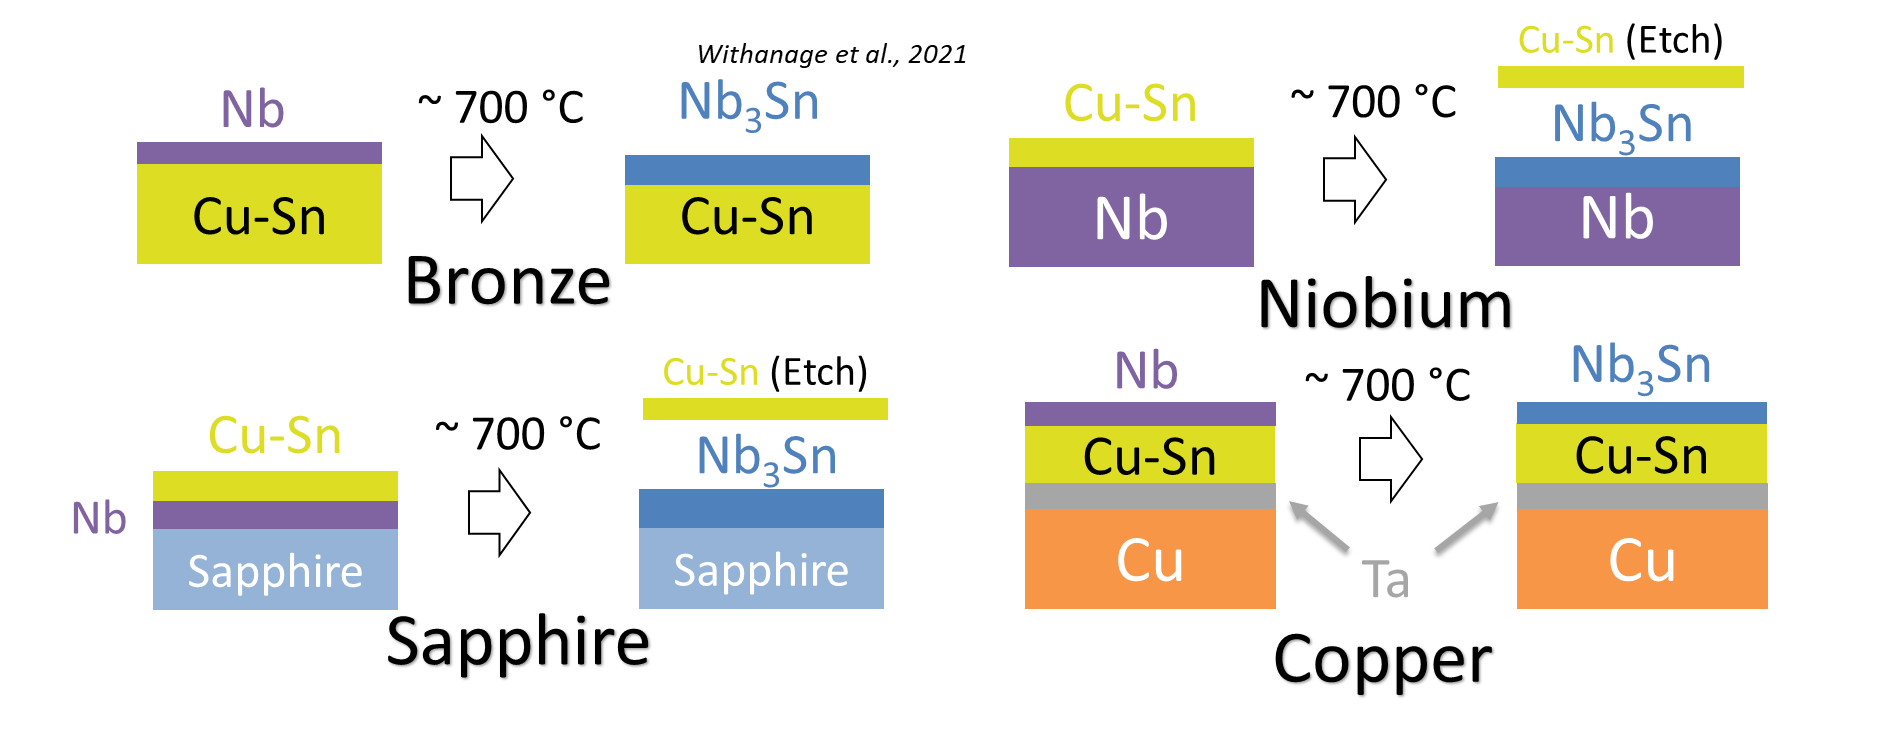
\includegraphics[width=.9\textwidth]{images/Nb3Sn/SubstrateSchematic.png}
    \caption{Schematic showing the different multilayers needed for Nb$_3$Sn reaction on bronze, Nb, sapphire, and Cu substrates.}
    \label{fig:SubstrateSchematic}
\end{figure}  

This chapter also reports multiple proof-of-principle studies to downselect three recipes with the most potential. Two recipes using the hot-bronze technique (see Sec:~\ref{sec:ourworkdescribe}) were separately achieved: (1) $\Delta T_c< 1$~K transitions proving compositional uniformity, and (2) $T_c = 17.7$~K demonstrating that strain can be managed through film thickness. Recipe (3) achieved an exceptionally uniform film morphology using an Nb-first post-reaction approach and was therefore selected as the RF cavity coating recipe in the next chapter.

%Our Nb substrate experiment allowed us to isolate the Nb-Sn reaction without the Cu bulk substrate sucking out Sn from the reaction front. The Nb substrate has a thermal expansion comparable to that of Nb$_3$Sn, so with a Nb substrate, the mismatch strain between the film and the substrate is minor. Any depression in $T_c$ is from low Sn content, a martensitic transition~\cite{battermanDynamicalDiffractionRays1964a}, and/or residual strain from defect formation during growth. 

%We present different deposition and heat treatment approaches, each using bronze compositions rich in Sn~\cite{yamasakiFabricationNb3SnSuperconductors1982a} to make high Sn high $T_c$ Nb$_3$Sn films. Preliminary experiment used Cu-Sn alloys with high Sn wt\% on niobium and sapphire substrates. We report superconducting properties and microstructural analyses for these routes. 

\section{Constraints on the Experiments}

Constraints on the temperature and time of heat treatments were enforced when reacting using the thin-film sputtering chamber. While this chamber provides excellent vacuum conditions ($10^{-9}$~torr at room temperature, degrading to $\sim10^{-7}$~torr at $750~^\circ$C due to outgassing), superior to the available tube furnace ($10^{-5}$ to $10^{-6}$~torr), heat treatments were restricted to 6 hours and a maximum temperature of $750~^\circ$C to prevent thermal damage to the chamber components. Samples may have achieved better phase purity and homogeneity with longer annealing times or higher reaction temperatures, which represents an avenue for future improvement. Additionally, the homogeneity of the Cu-Sn film could have been improved if the thermal evaporator had been equipped with substrate rotation and/or heating capabilities.

\section{Experimental Methods}

Experimental methods in thin film analysis and characterization is provided in Appendix~\ref{app:Methods}, useful for future graduate students in this field. Given here however, is a description of the specific methods used to fabricate and characterize the films made in this work.

    \subsection{Thin Film Fabrication}
    
    \subsubsection{Substrate Preparation}

    
    Single-crystal substrates (Si(100) and c-plane sapphire) were used as-received after standard ultrasonic cleaning in acetone and IPA. High-Sn bronze (13~wt.\% Sn), high-purity niobium, and oxygen-free high thermal conductivity (OFHC) copper were cut into 7.5x7.5 mm square samples from a 1 mm thick sheet using a guillotine blade. These substrates were mechanically polished to a mirror finish using progressive carbide paper ($400-1200$ grit), diamond slurry ($5-1$ \unit{\um}), and vibratory colloidal silica (0.05~\unit{\um}) polishing. Samples were ultrasonically cleaned in acetone and isopropyl alcohol (IPA) and stored in a desiccator until deposition.
    
    \subsubsection{Diffusion Barrier Deposition}
    
    The Cu substrates required diffusion layers before the Cu-Sn layer deposition. Without a diffusion barrier, too much Sn diffuses into the substrate, leading to poor-quality Nb$_3$Sn. A thick diffusion barrier can also allow for strain relaxation in the film. Diffusion-barrier materials with high melting points and high strength were used: $100 - 500$~nm-thick Ta, W, or Nb diffusion barriers. A 10 mTorr argon working gas was used for sputtering Ta and W, and 8 mTorr for Nb. All sputtering was done using a 5-target system manufactured by Kurt J. Lesker. The typical background pressure was $\sim 5 \times 10^{-9}$ Torr, and cryopumping enabled efficient removal of water and hydrogen. 
    
    The cleaned substrate was placed into the magnetron sputtering system, heated to 200~$^{\circ}$C for 10 minutes, and the diffusion barrier was sputtered onto the surface. After waiting for samples to cool, they were transferred into an Edwards Auto 306 Thermal evaporator with a base pressure of $\sim8 \times10^{-7}$ Torr using a liquid nitrogen-enhanced pump. The thermal evaporator was used to deposit Cu-Sn alloys. 
    
    %In the case of the Nb-first film, subsequently deposited the Cu-Sn layer onto this Ta/Nb multilayer and brought it back to the sputtering chamber for Cu. Then, they subsequently deposited the Cu-Sn layer onto this Ta/Nb multilayer and brought it back to the sputtering chamber for a post-reaction. For the Cu-Sn first film, we deposited a Ta diffusion barrier, transferred it from the vacuum to the thermal evaporator to deposit a Cu-Sn film, then returned it to the sputter chamber for Nb deposition and heat treatment.

    \subsubsection{High Sn\% Cu-Sn Alloys}

    Cu (99.9\% purity) and Sn (99.8\% purity) spherical powders (Alfa Aesar) were mixed to create four Cu-Sn compositions: 7, 14, 21, and 26~at.\% Sn. When these compositions were heated and vaporized, the resulting deposited film was single-phase or multiphase, depending on the initial composition. Cu-Sn films were made at thicknesses of 2, 5, and 10 \unit{\um}. Initially, a tungsten boat was used, but it resulted in very Sn-poor Cu-Sn films. A switch was made to alumina-coated tungsten baskets from R.D. Mathis for the remaining films. 
    
    \noindent The required Cu-Sn configuration depends on the substrate:
    
    \begin{itemize}
        \item \textbf{Nb substrates:} Cu-Sn deposited directly on Nb (no diffusion barrier needed)
        \item \textbf{Bronze substrates:} No additional Cu-Sn layer required---the substrate itself serves as the Sn reservoir  
        \item \textbf{Cu substrates:} Cu-Sn deposited on a diffusion barrier (Ta, Nb, or Mo) to prevent Sn loss into bulk Cu
    \end{itemize}
    
    \noindent This leads to two processing routes on Cu substrates:
    
    \begin{itemize}
        \item \textbf{Cu-Sn-first route:} Cu/Barrier/Cu-Sn/Nb $\rightarrow$ enabling a hot-bronze reaction and/or a post-reaction optimization after deposition
        \item \textbf{Nb-first route:} Cu/Barrier/Nb/Cu-Sn $\rightarrow$ only allows for a post-reaction (the thermal evaporation system was not equipped with a heater to facilitate in-situ reaction experiments)
    \end{itemize}
  
    Thermal evaporation enables rapid deposition of thick Cu-Sn films ($\sim$10 \unit{\um}/hour) with high purity and compositional control. When depositing materials with different vapor pressures and melting temperatures, such as Cu and Sn from the same thermal evaporation boat, composition gradients can develop across the film thickness during deposition (seen in Fig.~\ref{fig:CuSnGradient}). The substrate becomes hot due to radiative heating, causing diffusion during deposition that further alters the spatial distribution of Sn throughout the film. Since Sn redistributes during the subsequent Nb$_3$Sn formation reaction, these as-deposited composition gradients were not a primary concern for this application. 

    Poor wetting of the Cu-Sn layer on smooth substrates can lead to film dewetting and delamination. Two approaches were found to mitigate peeling: substrates with surface roughness $>10$~nm showed reduced delamination, and depositing Cu-Sn films in 5 steps at 20 \AA/s with 30-minute intervals between steps allowed for film cooling and strain relaxation, further reducing peeling. Both techniques were used in this study to mitigate Cu-Sn film peeling.
    
    %This can be achieved by stopping before perfect mirror polish.
    
    %wt\% Sn: Cu13Sn, Cu24Sn, Cu33Sn, and Cu40Sn = At%: Cu7Sn(alpha), Cu15Sn(alpha, beta, gamma), Cu21Sn(gamma + liqiud), and Cu26Sn(epsilon+eta)
    
    %\begin{figure}
    %    \centering
    %    
\includegraphics[width=.8\textwidth]{CuSnGradient}
    %    \caption{A Line scan shows the Sn concentration across the thickness of a thermally evaporated Cu-Sn film %on a Ta diffusion barrier with a Cu substrate. We observe a Sn gradient across the film thickness.}
    %    \label{fig:CuSnGradient}
    %\end{figure}
    %

    \begin{figure}[ht]
        \centering                
        
\includegraphics[width=.8\textwidth]{images/Cu/Diffusion/CuSnGradient.png}
        \caption[Thermally evaporated Cu-Sn film with concentration gradient.]{Thermally evaporated Cu-Sn film with concentration gradient. This gradient was found in the as-deposited film before reaction with Nb.}
        \label{fig:CuSnGradient}
    \end{figure}
    \FloatBarrier

    \subsubsection{Nb deposition and \texorpdfstring{Nb$_3$Sn}{Nb3Sn} reaction}

    The next step was deposition of Nb and Nb$_3$Sn reaction. The multilayer structure underwent a pre-heating step at 110~\unit{\celsius} in the sputtering chamber load lock to remove adsorbed water after transfer from the thermal evaporator to the sputter chamber. A Nb film was deposited using 8~mTorr working gas, 250~W power, and 0~V substrate bias. Three distinct recipes were employed:

    \begin{enumerate}
    
        \item Hot-Bronze: Nb deposited on heated Cu-Sn (650-750 °C) for the duration of the deposition process.
        \item Post-Reaction: Nb deposited at 200 °C, followed by in-situ heating (650-750 °C) for ~3 hours. 
        \item Hot-Bronze with Post-Reaction: Extended in-situ heating (650-750 °C) after the hot-bronze method. 
    
    \end{enumerate}
    
    \begin{figure}[ht]      
        \centering
        
\includegraphics[width=.7\textwidth]{images/Cu/CuMultilayer.png}
        \caption[A schematic representation of the Cu substrate with a diffusion layer and bronze beneath a Nb$_3$Sn film.]{A schematic representation of the Cu substrate with a diffusion layer and bronze beneath a Nb$_3$Sn film. This film is formed by hot- or cold-deposition of Nb, followed by a post-reaction. Notably, if Nb is deposited hot, it results in distinct microstructural differences and a higher $T_c$ onset due to the higher mobility of atoms at the elevated temperature. (Adapted from \citeauthor{withanageRapidNbSn2021})}
        \label{fig:CuMultilayer}
    \end{figure}

    \noindent The temperature recorded is inferred from a thermocouple nearby the sample, and therefore is not the input temperature from the furnace heating element.
    
    \subsection{Characterization Techniques}

        \subsubsection{Critical Temperature \texorpdfstring{$T_c$}{Tc}}

        Measurements of magnetic moment [emu] vs.\ temperature [K] were collected using a superconducting quantum interference device (SQUID) magnetometer (Quantum Design MPMS); Appendix~\ref{app:Methods} discusses the theory of operation and mounting technique. Samples with cross-sections no larger than $7.5 \times 7.5$~mm and a thickness of 2~mm were zero-field cooled below $T_c$, and any trapped flux was removed using the manufacturer's oscillatory degauss procedure. A 1~mT field was then applied parallel to the film surface to minimize demagnetization effects. The magnetic moment was measured in $\sim$0.1~K steps as the sample warmed to 20~K.
        
        The $T_c$ onset is defined as the last measured point before the normalized magnetic moment reaches zero, representing the highest-quality superconducting region in the film. The transition width $\Delta T_c$ is determined from the 90\%--10\% span of the superconducting transition, and the baseline is established by extrapolating the normal-state response. A narrow $\Delta T_c$ indicates uniform Sn stoichiometry throughout the film.
        
        However, $T_c$ measurements alone do not fully predict RF performance: they lack spatial resolution, are influenced by magnetic screening, and do not distinguish where high-quality Nb$_3$Sn resides within the film thickness. Microstructural characterization is therefore required to complement these results.
        
        \subsubsection{Microanalysis}

        %For Nb$_3$Sn characterization, 5--10~kV was used for surface morphology imaging and 15--20~kV for compositional analysis via EDS. 
        
        %A Rigaku SmartLab system was used to acquire X-ray diffraction (XRD) spectra to understand what crystal structures are in the film. 
        
        An FEI Helios G4 UC field-emission scanning electron microscope (SEM) with a focused ion beam (FIB) was used to study the surface and cross-sectional morphology in secondary-electron (SE) mode. The elemental composition with a spatial resolution of $\sim1$~\unit{\um} was analyzed using energy-dispersive spectroscopy (EDS) with an Oxford Instruments X-MaxN SDD x-ray detector and standardless analysis in the same SEM/FIB chamber. Roughness was measured using a DSX optical microscope, with a height resolution of less than 1~\unit{\um}. The piezoelectric stepper motors in the optical microscope allow for height resolution significantly better than its lateral resolution (limited by the wavelength of light).
        
        The film cross-section was also prepared (when a larger area was needed than FIB could provide) by slicing the coupon samples with a precision diamond saw perpendicular to the film and gluing the halves. A thermally evaporated silver film was deposited on the Nb$_3$Sn film surface to protect it before slicing, thereby reducing saw-induced damage. This sandwiched thin film was placed in a conductive powder mount and mechanically polished to a mirror finish for SEM analysis.

\section{Systematic Studies}

    In this section, the results of reactions between Nb and Cu-Sn under different conditions are provided. Specifically, these experiments helped determine the impact of strain from other substrates and neighboring layers near the Nb$_3$Sn film, as well as the effect of Sn concentration and mobility on the resulting Nb$_3$Sn properties. These experiments led to an optimized recipe for the RF cavity experiment, allowing further thin film characterization with quality factor measurements.

    \subsection{Sapphire Strain Experiment}\label{sec:SapphireExp}

    Initial analysis on bronze substrates experiments~\cite{withanageRapidNbSn2021}, found a depression of critical temperature by $\sim3~$K for the hot-bronze films, even when the Sn content was near maximum (26\%). Using XRD and COMSOL, the strain was determined to be dominated by CTE, with some additional strain from the growth mode. Since strain significantly affects superconducting properties in Nb$_3$Sn, a new experiment was designed to measure the $T_c$ of a film under three different strain conditions. Strain in the film resulted from thermal contraction mismatch between the sapphire substrate, Nb$_3$Sn film, and Cu-Sn layer. To isolate the contributions from each component, three sample states were characterized: (1) as-deposited film on sapphire, (2) film peeled from sapphire, and (3) film peeled and etched to remove the Cu-Sn layer.

    A 2~\unit{\um} Cu-13~at.\% Sn film was thermally evaporated in steps with 30-minute cooling intervals between each 1~\unit{\um} increment at a base pressure of $\sim3\times10^{-7}$ Torr onto a c-plane sapphire substrate. The Nb was then sputtered at 0.37~nm/s using 250~W power, 8~mTorr argon working gas, and a substrate temperature of 680~$^\circ$C with no pre-heat treatment.

    This presented an opportunity to compare different strain states due to thermal contraction mismatch from different layers, since the thermal contraction of sapphire is close to that of Nb$_3$Sn~\cite{eastonPredictionStressState1980}, and Cu-Sn CTE is significantly higher than either (Fig.~\ref{fig:CTECuNbNb3Sn}). $T_c$ before and after peeling from the sapphire substrate, leads to a critical temperature onset decrease from 17.11~K (black curve) to 16.77~K (blue curve Fig.~\ref{fig:SapphireStrain}). We attribute this to an increased strain impact from the nearby Cu-Sn layer, with the sapphire substrate mitigating the compressive strain in the Cu-Sn film. After peeling, the thin Cu-Sn/Nb$_3$Sn bi-layer was etched to study the impact the 2~\unit{\um} Cu-Sn film had on the Nb$_3$Sn layer, and found an increase of $T_c$ onset by almost 1~K (red curve Fig.~\ref{fig:SapphireStrain}). A Nb transition also appeared after etching, suggesting that the Cu-Sn layer removed some Nb$_3$Sn material that magnetically screened the Nb from the SQUID measurement. This study reveals that the residual Cu-Sn film beneath the Nb$_3$Sn layer induces sufficient strain to depress $T_\text{c,onset}$ by $\sim$1~K. Additionally, etching uncovered unreacted Nb and Sn-poor Nb$_3$Sn phases that were magnetically screened in initial SQUID magnetization measurements, which indicates hidden inhomogeneities in the film composition.

    \begin{figure}
        \centering
        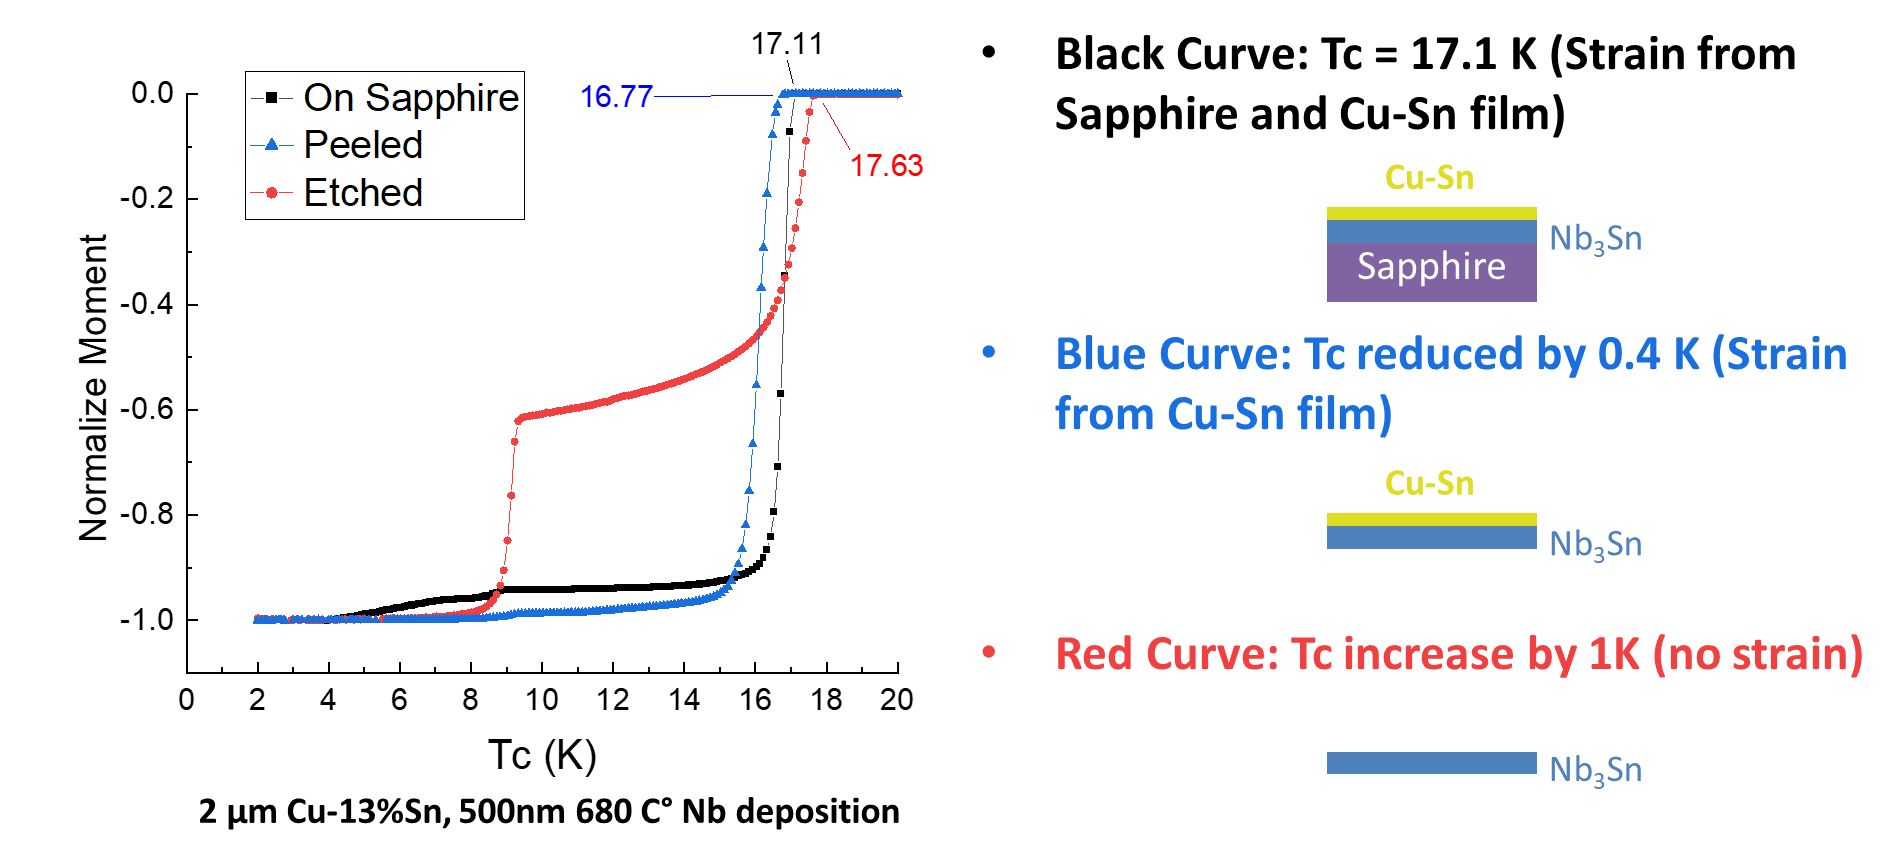
\includegraphics[width=.9\textwidth]{images/Sapphire/SapphireStrain.png}
        \caption{$T_c$ curves for a hot bronze film on sapphire, that has been peeled, and etched and measured at each stage.}
        \label{fig:SapphireStrain}
    \end{figure} 
    \FloatBarrier

    \subsection{Substrate Experiments}\label{sec:substratestrainandSn}

    By understanding the impact the substrate has on $T_c$, the effects of low Sn concentration and strain on superconducting performance can be separated. All samples used 2~\unit{\um} Cu-13~at.\% Sn films thermally evaporated in steps with 30-minute holds, followed by 500~nm Nb sputtered at 0.37~nm/s (250~W, 8~mTorr) at 680~$^\circ$C substrate temperature, with no additional pre- or post-heat treatment. This recipe matches the sapphire substrate conditions from Section~\ref{sec:SapphireExp}. These film conditions were chosen because they represent a minimum: low Sn volume in the Sn source and a relatively low reaction temperature. When Sn conditions are poor, strain and Sn effects are more readily observed.

    %Starting with the sapphire substrate (green curve in Fig.~\ref{fig:SubstrateExpTc}), we observe a high critical temperature onset around 17~K, and a very sharp transition. The high $T_c$ onset indicates a high Sn concentration and a low strain, with the sharp transition indicating a homogenous film. Next, the Nb $T_c$ curve has a profile similar to that of the sapphire substrate, but is shifted to 15~K. Like sapphire, Nb has a CTE similar to that of Nb$_3$Sn, so we can assume that the decrease in $T_c$ (blue curve in Fig.~\ref{fig:SubstrateExpTc}) is due to changes in Sn concentration and not from strain. In this geometry, with a Nb substrate and a Nb deposition, there are two Nb sources, leading to two different reactions: Nb$_3$Sn formation at the substrate and Nb$_3$Sn formation with the incoming hot Nb flux. In this experiment, there was a finite Sn volume in the thin 2~\unit{\um} Cu-Sn film and a high Nb volume from the substrate and deposition. Therefore, the resulting Nb$_3$Sn must have low-Sn activity, which explains the lower critical temperature compared to the sapphire substrate sample.

    Starting with the sapphire substrate (green curve in Fig.~\ref{fig:SubstrateExpTc}), a high critical temperature onset around 17~K with a very sharp transition was observed. The high $T_\text{c,onset}$ indicates high Sn concentration and low strain, with the sharp transition indicating film homogeneity. 

    In contrast, the Nb substrate sample (blue curve) exhibited a similar transition profile but was shifted downward to 15~K. Since Nb has a CTE similar to Nb$_3$Sn (Fig.~\ref{fig:CTECuNbNb3Sn}), the decreased $T_c$ can be attributed to reduced Sn concentration rather than strain effects. For the Nb substrate geometry, two Nb sources are present during the reaction: the Nb substrate itself and the deposited Nb film. This creates competing reactions for Nb$_3$Sn formation at both the substrate interface and within the deposited layer. With a finite Sn supply from the thin 2~\unit{\um} Cu-Sn film and excess Nb from both sources, the resulting Nb$_3$Sn is Sn-deficient, explaining the reduced critical temperature compared to the sapphire substrate sample.
    
    Moving to the Cu substrate with a Ta diffusion barrier (red curve in Fig.~\ref{fig:SubstrateExpTc}) sample, a further reduction in $T_c$ onset to 12 K and a broad transition was seen. This was due to significant strain from the Cu substrate and a medium Sn content. The Ta diffusion barrier blocks some Sn from migrating into the Cu substrate; however, because the original Sn content is low, this results in a tin deficiency in the Nb$_3$Sn layer. The adverse effects of the Cu substrate are even further pronounced when no Ta diffusion barrier is present, and no Sn is blocked from entering the Cu substrate, as is the case with the black curve in Fig.~\ref{fig:SubstrateExpTc}. The $T_c$ onset further decreases to 10 K, almost at the Nb transition, indicating very low Sn concentration and a considerable strain from the Cu substrate. 

    \begin{figure}[tb]
        \centering
        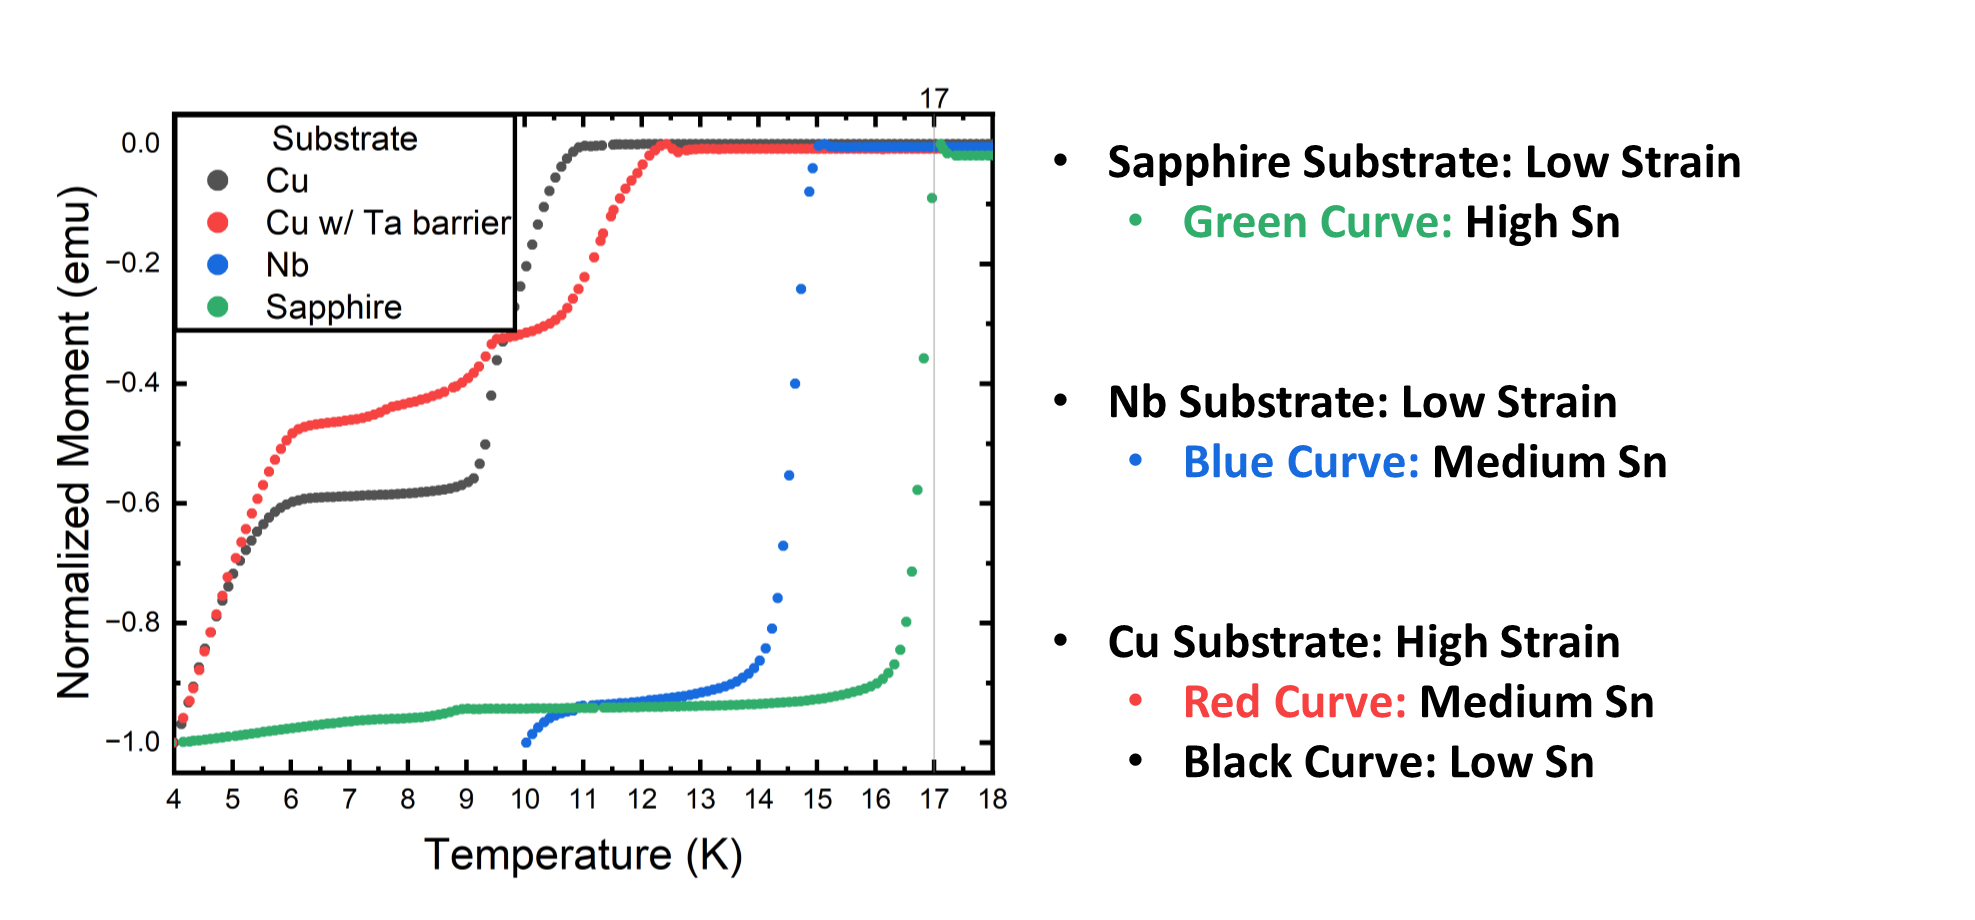
\includegraphics[width=\textwidth]{images/Nb3Sn/SubstrateExpTc.png}
        \caption{$T_c$ curves for substrates: Cu, Cu w/ Ta diffusion barrier, Nb, and sapphire.}
        \label{fig:SubstrateExpTc}
    \end{figure}  
    \FloatBarrier

    \subsection{Nb Substrate - High Sn Cu-Sn}\label{sec:Nbsub}

    The following Nb substrate experiment varied the Sn content in the Cu-Sn films (Fig.~\ref{fig:SourcevsFilmCuSn}) and heat-treatment profiles to determine an optimal recipe determined by the critical temperature (Fig.~\ref{fig:NbSubTcandSChem}). All of these films used a post-reaction method to convert Nb into Nb$_3$Sn. 

    \begin{figure}[htb]
        \centering
        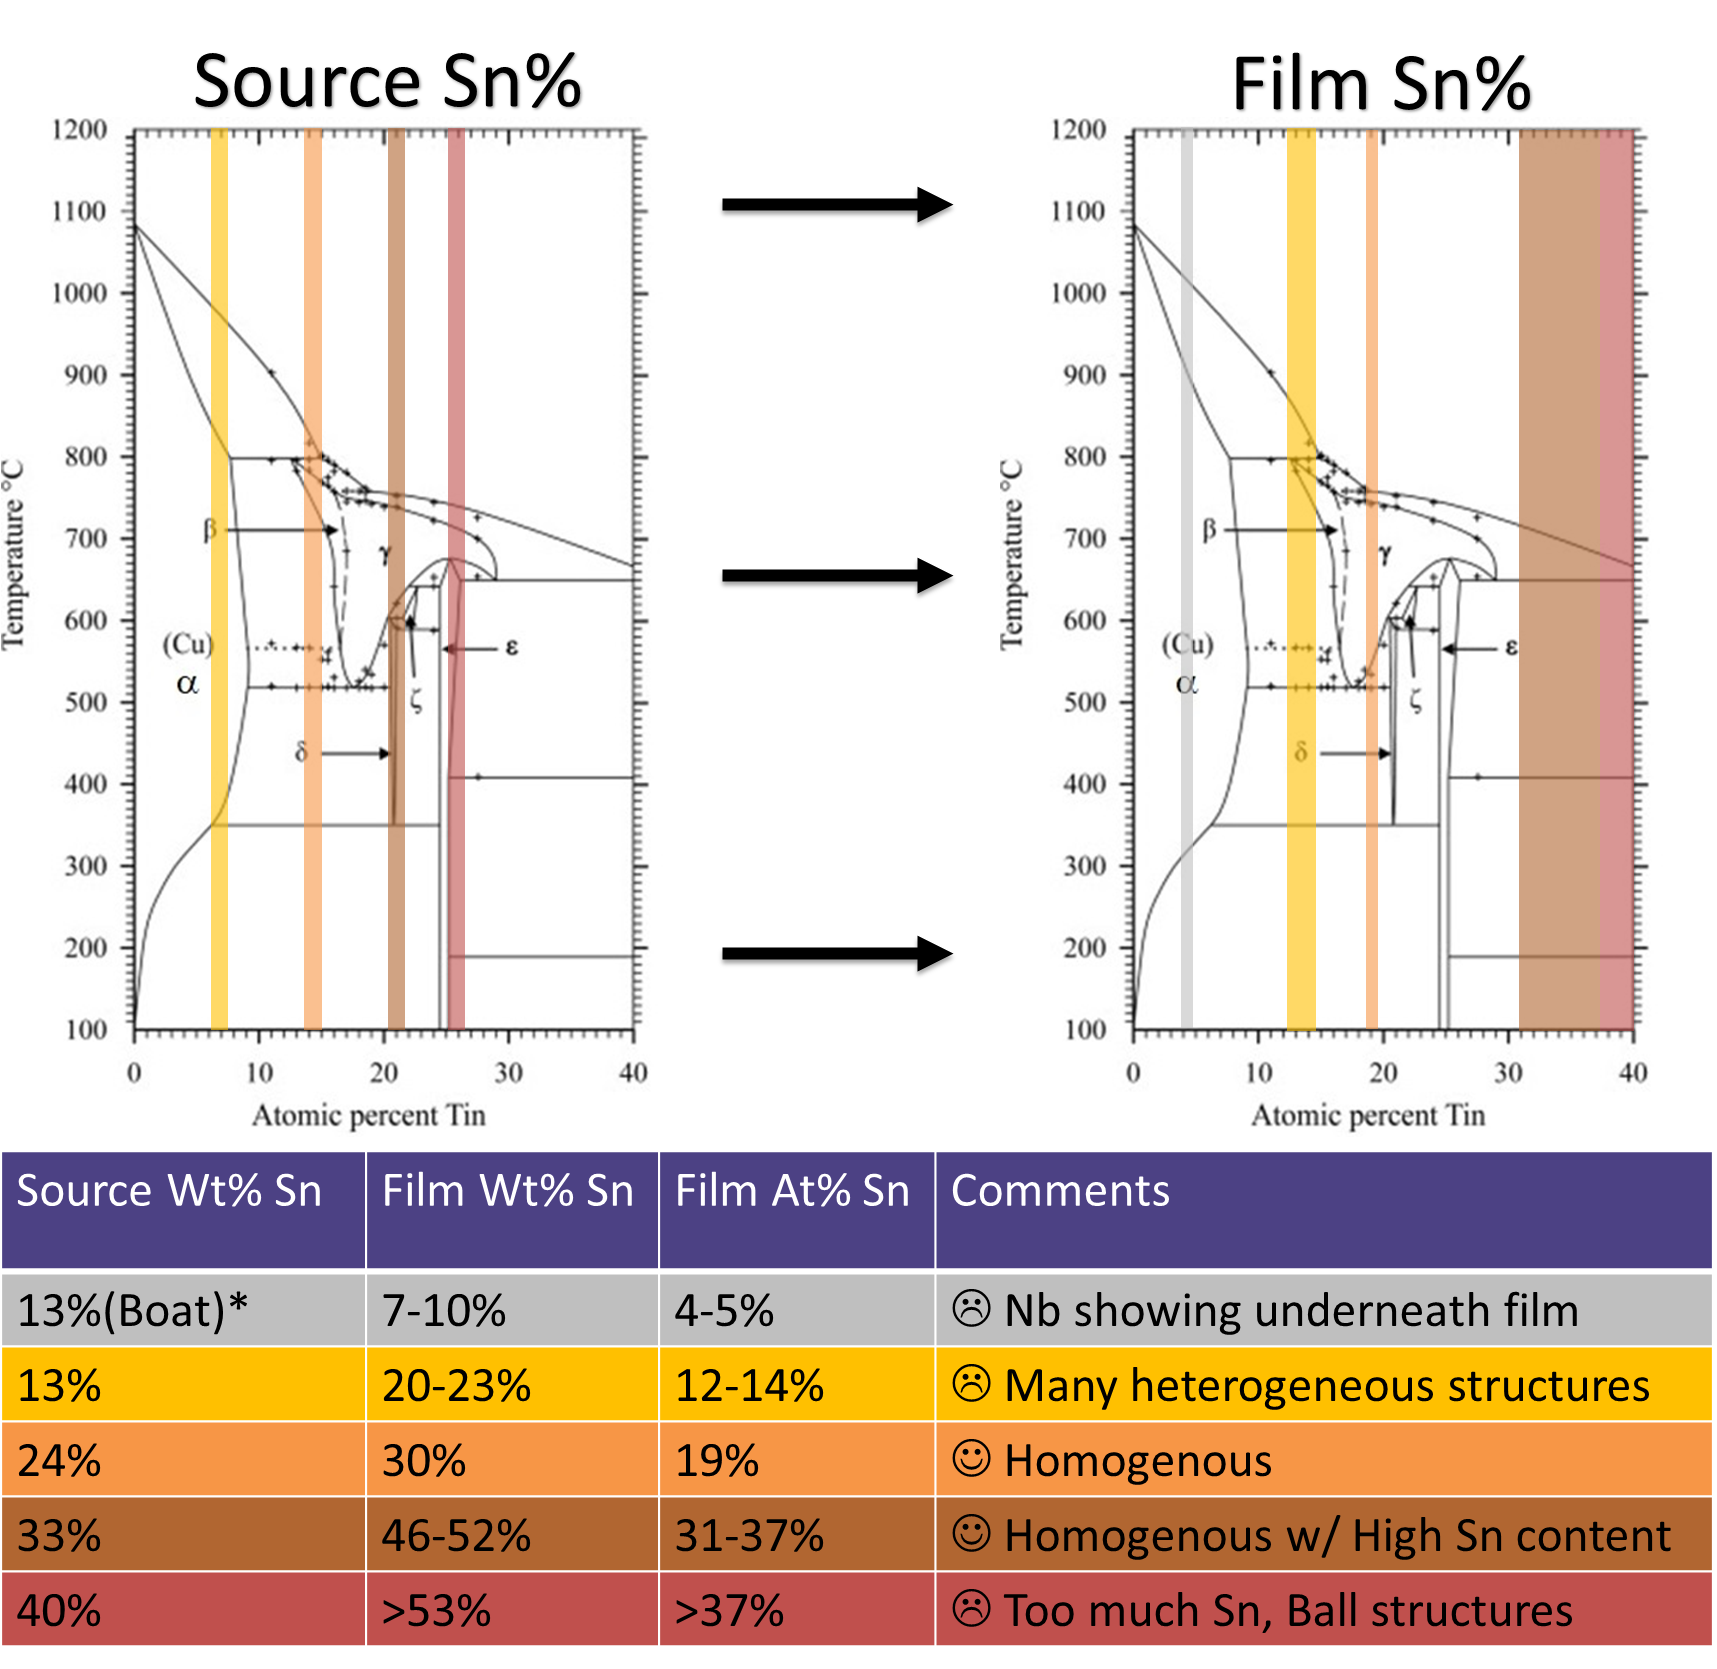
\includegraphics[width=.9\textwidth]{images/Nb/SourcevsFilmCuSn.png}
        \caption{Cu-Sn phase diagram showing initial source Sn concentration and final Cu-Sn layer Sn concentration, with a comment on resulting microstructure.}
        \label{fig:SourcevsFilmCuSn}
    \end{figure}
    \FloatBarrier


    
    Cu-Sn films with five different compositions (4, 13, 19, 33, and 37~at.\% Sn as measured by EDS after deposition and top surfaces images in Fig.~\ref{fig:BronzeOnNbSnVariation}) were thermally evaporated onto Nb substrates to a thickness of 4~\unit{\um}, deposited in four 1~\unit{\um} steps with 30-second holds between steps to allow for film cooling and strain relaxation. The thermal evaporator base pressure was $\sim3\times10^{-7}$ Torr before deposition. These samples were then transferred to a positive-pressure argon furnace equipped with a PPM oxygen filter and ultra-high-purity (UHP) argon gas at a flow rate of 0.2 L/min. The furnace was pumped down to $4\times10^{-5}$ Torr before introducing argon flow. The furnace was ramped at 10~$^\circ$C/min to the reaction temperature. Heat treatments were performed at 650, 700, and 750~$^\circ$C for either 12 or 24 hours, testing all five Sn compositions at each temperature and time combination (30 samples total). The Nb$_3$Sn formation occurred entirely within this tube furnace; no sputtering chamber processes were used for this experiment.

    
    \begin{figure}[htb]
        \centering
        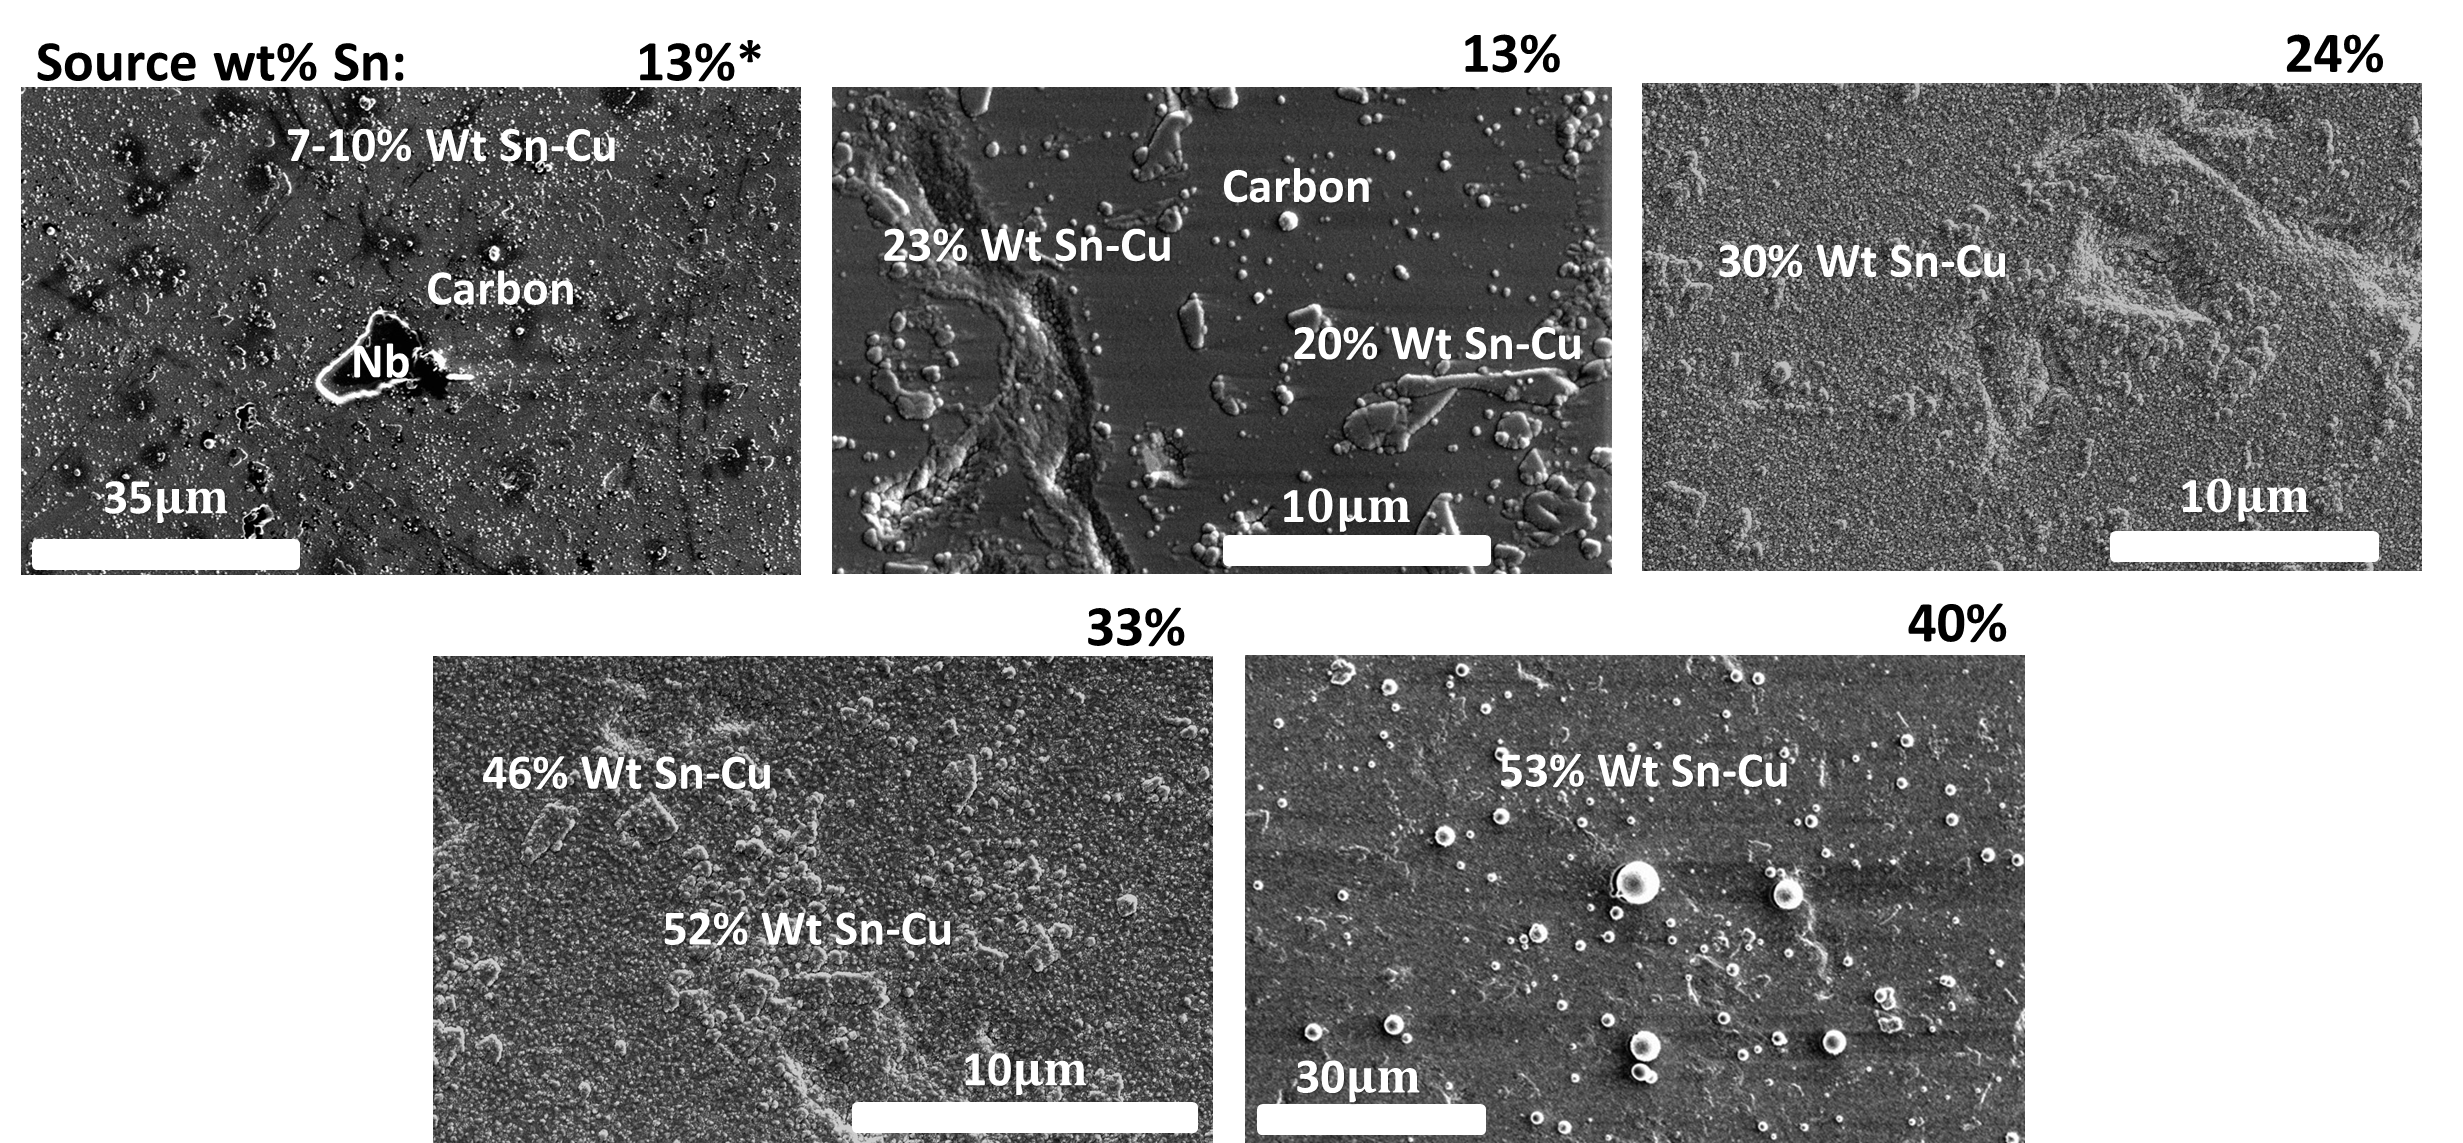
\includegraphics[width=\textwidth]{images/Nb/BronzeOnNbSnVariation.png}
        \caption{4 \unit{\um} Cu-Sn films with varying Sn content on Nb substrates.}
        \label{fig:BronzeOnNbSnVariation}
    \end{figure}

    



    
    Higher temperature consistently increased the critical temperature, given our reaction temperatures of $650 - 750$ $^\circ$C (Fig.~\ref{fig:NbSubTcandSChem}). This is consistent with observations in literature, which showed increased Sn mobility at elevated temperatures leading to an increased Sn content in the Nb$_3$Sn~\cite{chadmatthewfischerINVESTIGATIONRELATIONSHIPSSUPERCONDUCTING2002, hawesMeasurementsMicrostructuralMicrochemical2006, nausOptimizationInternaltinNiobiumtin2002, godekeReviewPropertiesNb3Sn2006, pongCuDiffusionNb3Sn2013}. Little change was observed in the superconducting properties between 12- and 24-hour reactions, except that the 24-hour reaction yielded a thicker Nb$_3$Sn layer. The separate tube furnace with positive-pressure argon was used for these experiments, enabling longer heat-treatment times.

    The Sn concentration plotted on the x-axis of Fig.~\ref{fig:NbSubTcandSChem} represents the composition of the deposited Cu-Sn film (measured by EDS after deposition), which differed from the starting powder composition in the evaporation boat. This is due to the difference in Sn and Cu vapor pressure, as explained in Appendix~\ref{app:Methods}. The lowest Sn concentration film (7~wt.\% Sn) was produced using the 13~wt.\% Sn starting powder, and the uncoated tungsten boat. The remaining Cu-Sn concentrations were fabricated using the alumina-coated tungsten boats.
    
    %instead of alumina-coated boats. This resulted in excessive Sn loss during evaporation, yielding an unexpectedly Sn-poor film.
    
    An optimal Sn concentration range for the final deposited Cu-Sn layer was found to be between 30 and 46~wt.\% Sn. Below 30~wt.\% Sn, the Cu-Sn reservoir could not supply sufficient Sn during reaction, producing Sn-depleted Nb$_3$Sn with reduced $T_c$. Above 46~wt.\% Sn, the Cu-Sn film exhibited very rough surface morphology, creating spatial inhomogeneities in Sn availability. This non-uniform reaction produced regions with varying Nb$_3$Sn stoichiometry, broadening the transition and depressing the $T_c$ onset.
    
    Note that these $T_c$ measurements were performed without etching away the Cu-Sn layer after reaction. As demonstrated in the sapphire substrate experiments (Section~\ref{sec:SapphireExp}), residual Cu-Sn can affect measured $T_c$ values due to strain effects, though the compositional trends observed here remain valid.

    \begin{figure}[H]
        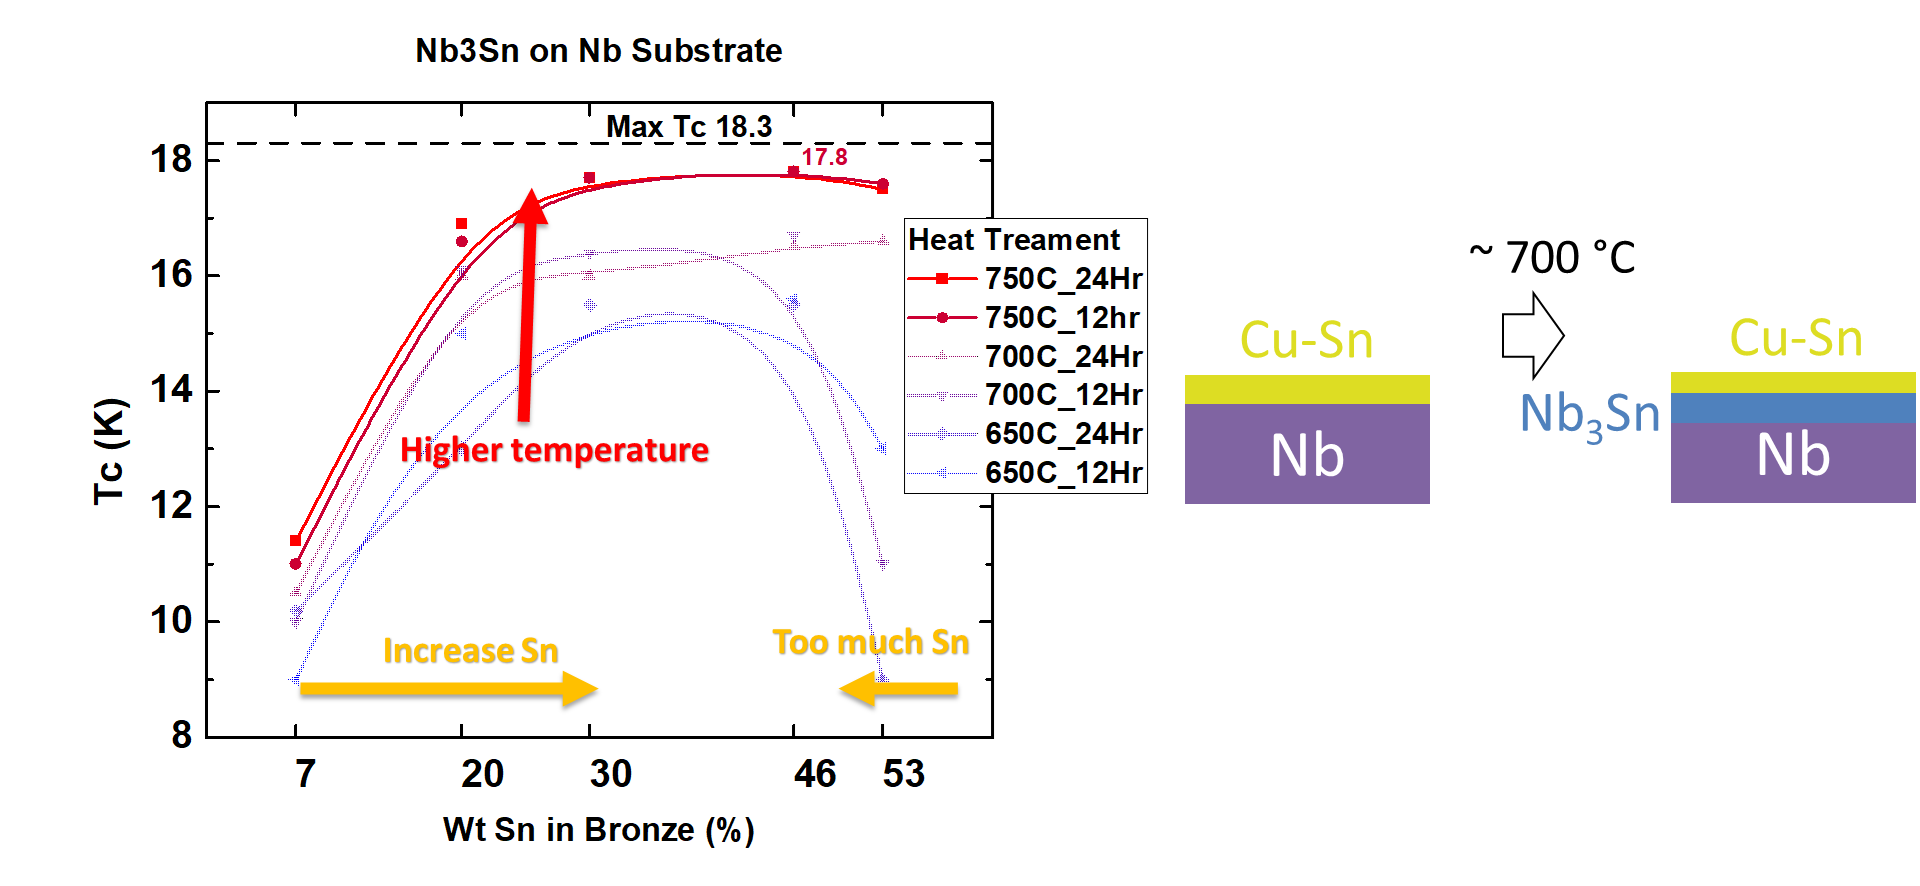
\includegraphics[width=\textwidth]{images/Nb/NbSubTcandSChem.png}
        \caption{$Tc$ curves for Nb$_3$Sn films Nb substrates made with varying Sn content, Cu-Sn films, and heat-treatment profiles.}
        \label{fig:NbSubTcandSChem}
    \end{figure}
    \FloatBarrier
    

    \subsection{High-Sn Routes Combined with Cu Substrates}

    The final proof-of-principle experiment aimed to understand how the Sn concentration in the final Nb$_3$Sn film was affected by the Cu substrate. This experiment used three different Cu-Sn starting powder concentrations (13, 24, and 33~wt.\% Sn) thermally evaporated to 5~\unit{\um} thickness in 1~\unit{\um} steps with 30-second holds between steps. A 500~nm Ta diffusion barrier was first sputtered onto the Cu substrate at 200~$^\circ$C. The Cu-Sn layers were deposited via thermal evaporation at a base pressure of $\sim4\times10^{-9}$ Torr. After a 110~$^\circ$C, 10-minute load lock preheat, 300~nm of Nb was sputtered at 0.37~nm/s using 250~W power and 8~mTorr argon working gas (802~s total deposition time). Three reaction profiles were tested: (1) \textbf{hot-bronze}: Nb deposited at 715~$^\circ$C with 30-minute substrate preheat, no post-reaction; (2) \textbf{post-reaction}: Nb deposited at 200~$^\circ$C, followed by 715~$^\circ$C heat treatment for 4 hours; and (3) \textbf{hot-bronze + post-reaction}: Nb deposited at 715~$^\circ$C with 30-minute preheat, followed by an additional 715~$^\circ$C heat treatment for 3 hours after deposition was completed.
    
    A schematic of the multilayer and all $T_c$ curves is given in Figure~\ref{fig:Nb3SnCuSubSnconcentration}. The prior work on Nb substrates identified 33 wt.\% Sn as optimal for achieving high $T_c$. This experiment again confirmed that 33 wt.\% Sn in the Cu-Sn layer was optimal, verifying for Cu substrates as well, across the full composition range: 13 wt.\% Sn produced $T_c \sim 11$~K, 24 wt.\% Sn yielded $T_c \sim 13$~K, and 33 wt.\% Sn reached $T_c \sim 16$~K. The hot-bronze + post-reaction process achieved the highest critical temperatures and sharpest transition. The reduction in $T_c$ by $\sim 2$~K from the ideal 18~K, is mainly due to the CTE mismatch between the Nb$_3$Sn and the Cu substrate.

    %back up by simulation and theory
    
    \begin{figure}[H]
        \centering
        
\includegraphics[width=\textwidth]{images/Cu/Nb3SnCuSubSnconcentration.png}
        \caption{(a) $T_c$ curves for Nb$_3$Sn on Cu substrates with varying reactions and Sn concentrations, and (b) a schematic showing the multilayer structure.}
        \label{fig:Nb3SnCuSubSnconcentration}
    \end{figure}  

    \section{Implications of the Proof-of-Principle Experiments for High-Quality \texorpdfstring{Nb$_3$Sn}{Nb3Sn} Films}

    \subsection{Hot-Bronze + Post-Reaction}\label{sec:2StepProcess}

    The hot-bronze deposition method, where Nb is sputtered at 715~°C onto Cu-Sn, offers rapid Nb-Sn reaction kinetics, approximately 12× faster than with post-reaction alone, and results in a higher initial Sn content~\cite{withanageRapidNbSn2021}. In this work, to enable hot-bronze films on Cu substrates, a Ta/Cu-Sn multilayer was deposited on a Cu substrate. The high substrate temperature provides thermal energy for immediate reaction as Nb atoms arrive at the Cu-Sn surface. As the Nb$_3$Sn film thickness increases with longer deposition time, Sn concentration at the surface appears to deplete. To address Sn depletion, a post-reaction heat treatment of 3 hours at 715~°C helped saturate Sn throughout the Nb$_3$Sn film by grain-boundary diffusion. During this step, Sn redistributes into Sn-deficient regions of the Nb$_3$Sn film, making it more homogeneous. 
    
    Post-reaction alone can also produce $\sim1$~\unit{\um} thick Nb$_3$Sn films. However, based on the results for 3-hour reactions in Fig.~\ref{fig:Nb3SnCuSubSnconcentration}, there is evidently a sluggish start to the layer growth that is avoided by the hot-bronze deposition. 

    
    %The results is an initial Nb$_3$Sn layer with columnar grain structure (Zone 2 Thornton morphology~\cite{andersStructureZoneDiagram2010}) and non-uniform Sn distribution.
    
    

    Neither approach alone achieves optimal results for this configuration on Cu (an alternative for Cu-Sn on Nb is discussed later). The combination of an initial hot-bronze deposition followed by further annealing after the deposition is stopped enables both a high critical temperature onset and a sharp superconducting transition. This demonstrates that high-quality Nb$_3$Sn films can be fabricated on Cu substrates when using the Cu-Sn route.

   \begin{figure}
       \centering
       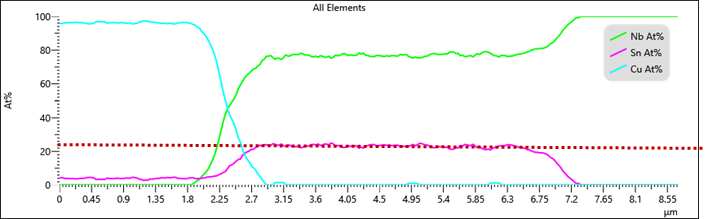
\includegraphics[width=.8\textwidth]{images/Cu/linescan25Sn.png}
       \caption{EDS showing the Sn content at 25\% at. Sn for one of our hot-bronze samples on a Nb substrate. The Nb substrate is to the right, and the surface of the film is to the left.}
       \label{fig:linescan25Sn}
   \end{figure}
    
    \subsection{Nb First or Cu-Sn first}

    \begin{table}[h]
        \centering
        \caption{Microstructural trade-offs for Cu-Sn layer position}
        \label{tab:CuSn_position_comparison}
        \begin{tabular}{lcc}
        \hline
        Property & Cu-Sn First & Nb First \\
        \hline
        Hot-bronze capable? & \ding{51} & \ding{55} \\
        Nb$_3$Sn thickness uniformity & Poor (follows rough Cu-Sn) & Excellent \\
        Ta/Nb$_3$Sn interface quality & Rough (via Cu-Sn) & Sharp (direct contact) \\
        Tc (onset) & 16K & 15K \\
        $\Delta$Tc & $<$1K & $\sim$2K \\
        Requires etching? & \ding{55} & \ding{51} \\
        \hline
        \end{tabular}
    \end{table}

    So far, all methods explored place the Cu-Sn layer and the Sn source below the Nb. This requires the reaction to convert the entire Nb layer, leaving Nb$_3$Sn on the RF-facing side of the cavity. However, in this situation, the RF-facing material would be farthest from the Sn source, and could thus be depleted in Sn. While the results in the prior sections show that the hot-bronze plus post-reaction approach is viable for $\sim500$~nm thick Nb$_3$Sn layers, it would still be preferable to ensure that the Sn-rich Nb$_3$Sn region is at the RF surface. As outlined in section~\ref{sec:ourworkdescribe}, an alternative approach is to deposit Cu-Sn on Nb or a suitably prepared Cu/Nb base material, react the layers after deposition to form Nb$_3$Sn, and then remove Cu-Sn by etching or electropolishing. 

    The Nb$_3$Sn film can be synthesized with the Sn source (Cu-Sn layer) positioned either underneath or on top of the Nb film. These two geometries each have distinct advantages and limitations.

    The hot-bronze reaction requires Nb atoms to arrive on a hot ($\sim715$~°C) Cu-Sn surface. This imposes a strict deposition order: Cu-Sn must be on the substrate and in the deposition chamber before Nb sputtering begins:

    \begin{itemize}
        \item \textbf{Cu-Sn first} (Fig.~\ref{fig:BronzeonNbandNbonbronzediagram}a): 
        Hot-bronze capable
        \item \textbf{Nb first} (Fig.~\ref{fig:BronzeonNbandNbonbronzediagram}b): 
        Hot-bronze impossible (Cu-Sn arrives after Nb already deposited)
    \end{itemize}


    \begin{figure}
        \centering
        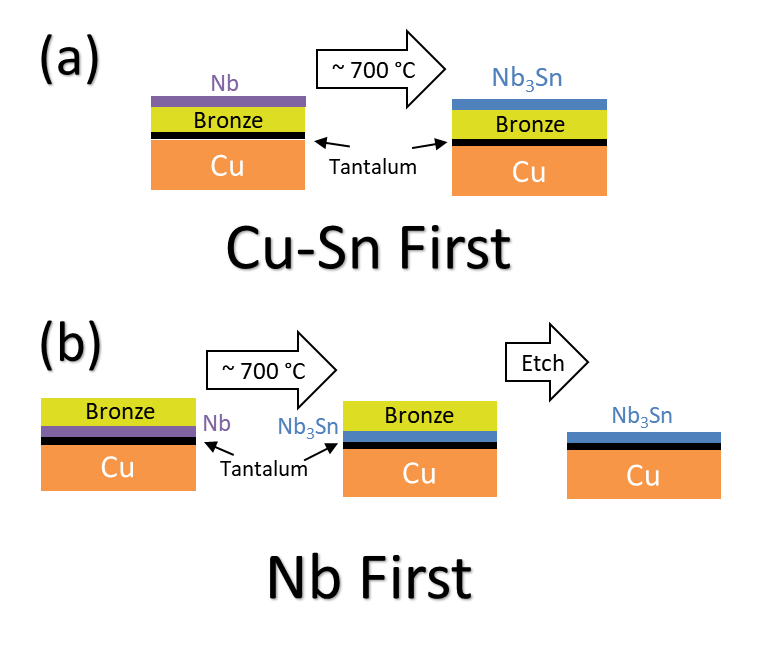
\includegraphics[width=.6\textwidth]{images/Cu/BronzeOnNb/BronzeonNbandNbonbronzediagram.png}
        \caption{Schematic showing (a) hot-bronze viable route Nb$_3$Sn on bronze, and uniform microstructure sample (b) bronze on Nb$_3$Sn requiring etching the Cu-Sn away after reaction.}
        \label{fig:BronzeonNbandNbonbronzediagram}
    \end{figure}        
  
   A plausible Nb-first route on a copper substrate would begin with a well-polished Cu surface, followed by a diffusion barrier (Ta) and, optionally, interface layers to improve adhesion and morphology. Fortunately, it was found that smooth Ta films adhered well when deposited directly on polished Cu. Subsequent deposition of Nb resulted in exceptionally uniform morphology. A sharp interface between Ta and Nb was observed with little to no oxidation (Fig.~\ref{fig:BronzeOnNb}). Large defects were not observed, unlike the porous layers sometimes observed for Cu-Sn layers ( seen in a) Fig.~\ref{fig:FullNb3Sn10micron2}). After sputtering Ta/Nb, Cu 33~wt.\% Sn was evaporated onto the Nb layer and reacted at $715~^\circ$C for 3 hours. After the reaction, the Cu-Sn was removed by etching in ammonium persulfate (APS). The resulting Nb$_3$Sn film displayed a $T_c$ of 15~K and $\Delta T_c$ of 2~K (blue curve in Fig.~\ref{fig:Recipe123Tc}). These properties are consistent with other Nb$_3$Sn films on Cu substrates.

    %Etching was found to affect the $T_c$ transition width ($\Delta$Tc increased from $<$1K to $\sim$2K), and the results are shown in the appendix.



    %\begin{figure}
    %    \centering
    %    
\includegraphics[width=.9\textwidth]{images/Cu/CuSnThickness/FullNb3Sn10micron.png}
    %    \caption[Full characterization of a Cu-Sn first film, including cross-sectional optical and SEM, EDS mapping, and EDS linescan]{Cu-Sn first film cross-sectional characterization: (a) optical micrograph and (b) SEM image showing the layered structure from Cu substrate through Ta diffusion barrier, bronze layer, Nb$_3$Sn film, and residual Cu-Sn alloys on top. The colored boxes in (a) and (b) indicate regions examined at higher magnification and with EDS analysis. (c) EDS elemental mapping of the cyan-boxed region showing spatial distribution of Nb, Sn, Cu, Ta, and Ag, along with the corresponding optical image. The Sn map reveals that Sn penetrated through the Ta diffusion barrier, with comparable Sn concentration on both sides of the Ta layer, indicating barrier failure. (d) High-magnification SEM image (top) of the orange-boxed region and corresponding EDS line scan (bottom) across the Nb$_3$Sn layer, showing approximately 25~at.\% Sn uniformly distributed across the film thickness. The non-uniform surface morphology and thickness variations of the Nb$_3$Sn film, visible in both (a) and (b), result from the underlying bronze layer's porosity and roughness. The optical image in (a) and EDS map in (c) also reveal multiple Cu-Sn alloy compositions near the Nb$_3$Sn surface, appearing as distinct phases with different optical contrast.}
    %    \label{fig:FullNb3Sn10micron}
    %\end{figure}
    %\FloatBarrier

    %\subsection{Cu-Sn layer Removal}

    %When using the Cu-Sn first method, Nb$_3$Sn is the final surface layer; etching is not needed. However, as with the Nb-first method, the final surface layer is not the high-Q layer (the superconducting layer), so etching is required to remove the Cu-Sn layer, revealing the Nb$_3$Sn layer as the final surface layer. Etching the Cu-Sn layer can change the critical temperature, as we have already seen in the sapphire experiment (Sec.~\ref{sec:SapphireExp}), and it can also affect the surface morphology. In this experiment, we tested the impact of etching on surface morphology and found it had minimal effect. We chose three methods for Cu-Sn surface-layer removal: nitric or ammonium persulfate (APS) acid etching and phosphoric acid electropolishing (EP). Among the enchants, nitric was abandoned because it was more aggressive than APS, leading to pitting. We found that both phosphoric acid EP and APS etching were easy to control and both provided adequate removal of the Cu-Sn film while leaving the Nb$_3$Sn film intact. The films shown below were etched with APS.

    A schematic of the multilayer is shown before and after etch, and includes a top-down 3-D optical image of the film (Fig.~\ref{fig:Nbsubetching}). The Cu-Sn film was selectively removed in one area by taping one side, since the etchant could not penetrate the tape. The same etched and non-etched film cross-section was analyzed (Fig.~\ref{fig:NbsubetchSEM}). The etched and non-etched sides show continuous Nb$_3$Sn throughout the film, verifying the success of the etching process.

    \begin{figure}[htb]
        \centering
        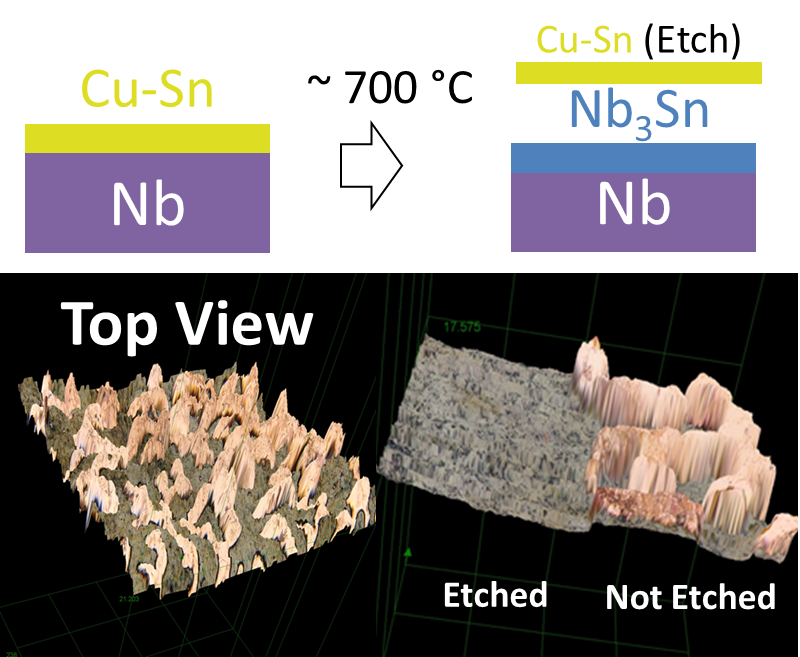
\includegraphics[width=.7\textwidth]{images/Nb/Nbsubetching.png}
        \caption{Schematic of the Nb$_3$Sn film on a Nb substrate, with a 3-D optical imaging showing the surface morphology before and after etching.}
        \label{fig:Nbsubetching}
    \end{figure}  

   \begin{figure}
        \centering
        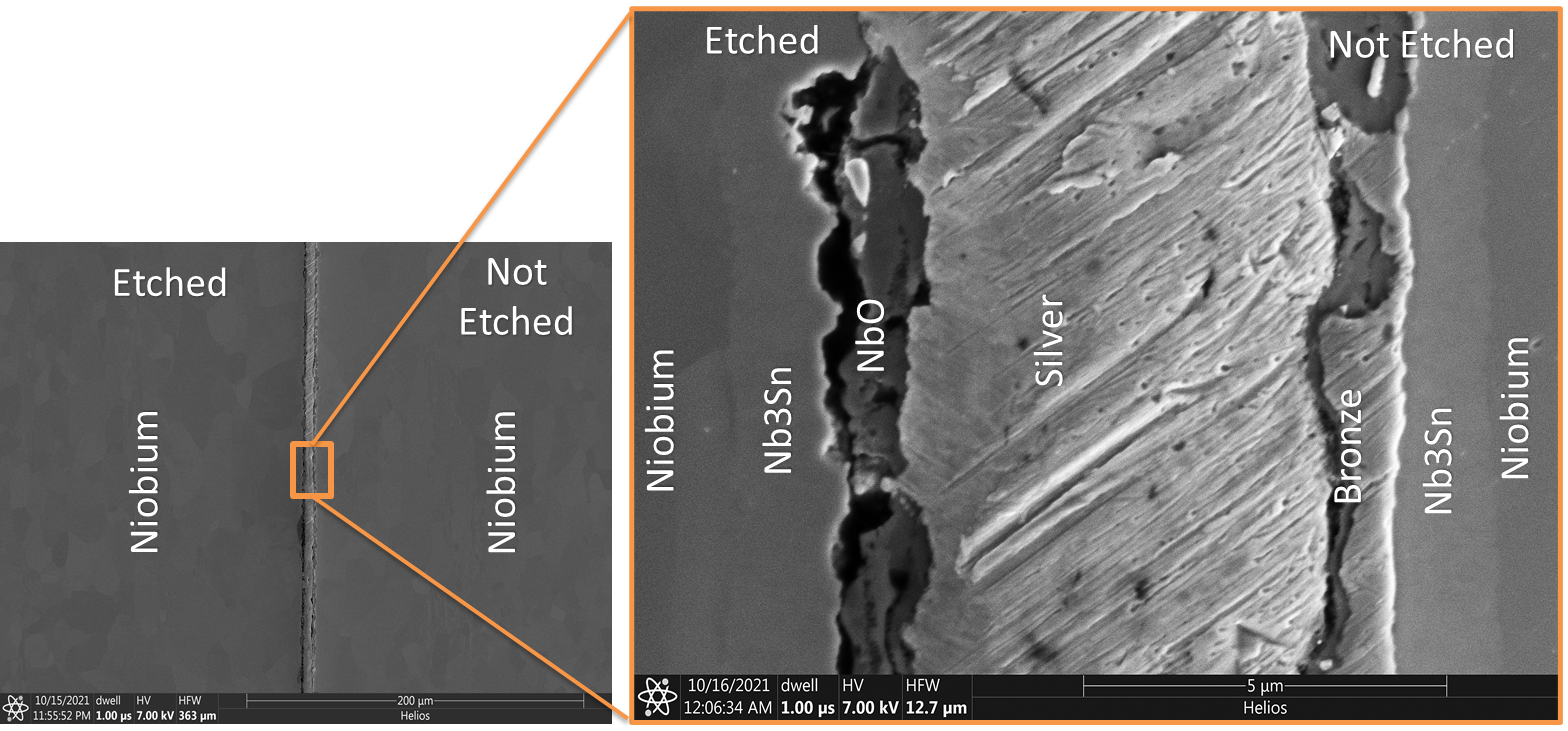
\includegraphics[width=.9\textwidth]{images/Nb/NbsubetchSEM.png}
        \caption[SEM images of a Nb$_3$Sn film on a Nb substrate that was cut in half, and one half was etched and the other half not etched, and sandwiched together]{SEM images of a Nb$_3$Sn film on a Nb substrate that was cut in half, and one half was etched and the other half not etched, and sandwiched together.}
        \label{fig:NbsubetchSEM}
    \end{figure}
    \FloatBarrier

    \section{Three Optimized Recipes for Cu Substrates}
   
    From the systematic studies on bronze~\cite{withanageRapidNbSn2021}, Nb, sapphire, and Cu substrates, three recipes were chosen optimized for $T_c$ (Fig.\ref{fig:Recipe123Tc}) and RF cavity application. 

    \begin{figure}[htb]
        \centering
        
\includegraphics[width=.7\textwidth]{images/Cu/Recipe123Tc.png}
        \caption[$T_c$ curves for best Nb$_3$Sn samples on Cu substrates.]{$T_c$ curves for best Nb$_3$Sn samples on Cu substrates. Black curve: Recipe 1 (thin Cu-Sn first) with sharp transition, $\Delta T_c \approx 1$~K. Red curve: Recipe 2 (thick Cu-Sn first) with the highest $T_c = 17.7$~K onset, but low-Sn Nb$_3$Sn near the surface. Blue curve: Recipe 3 (Nb first) with uniform morphology, but needing longer reaction.}
        \label{fig:Recipe123Tc}
    \end{figure}        
    
    %We identified key requirements for Cu-compatible processing:
    
    %\begin{itemize}
    %\item \textbf{Sn content:} 33 at.\% in Cu-Sn source (Nb and Cu substrate studies)
    %\item \textbf{Strain management:} CTE mismatch causes 2K depression; thicker films (>3\unit{\um}) partially relax
    %\item \textbf{Reaction pathway:} Hot-bronze enables high Sn concentration earlier in the reaction, and post-reaction saturates the Nb$_3$Sn stoichiometrically rains
    %\item \textbf{Nb first:} When Nb is directly deposited on Ta, the resulting Nb$_3$Sn film is very uniform
    %\end{itemize} 

    \subsection{Recipe 1: Thin Cu-Sn First}

    The superconducting transition (black curve in~\ref{fig:Recipe123Tc}) and microstructure (Figure~\ref{fig:300nmNb3sn16K}) of the most stoichiometrically uniform Nb$_3$Sn film on Cu are reported. This sample was made using a 500~nm Ta diffusion barrier, a 5 \unit{\um} Cu- 33~at.\% Sn film, then deposit 300~nm of Nb at 700 $^\circ$C, and post-react for 3 hours. This sample exhibited a $T_c$ onset of 16~K and a sharp transition of $\Delta T_c\sim1$ K. It is of note that a small amount of the film had a $T_c < 6$~K, which is not used for calculating $\Delta T_c$. The 0.9\% compressive strain estimated from the Cu substrate CTE mismatch (Fig.~\ref{fig:CTECuNbNb3Sn}) depresses $T_c$ by approximately 2~K (Fig.~\ref{fig:TcvsStrain}). A small $\Delta T_c$ indicates that the film is highly uniform in stoichiometry, owing to its thin width and ample Sn supply. Delamination and cracking were observed in the Cu-Sn layer, as seen with other Ta barrier films. This sample employed the hot-bronze + post-reaction two-step process described in Section~\ref{sec:2StepProcess}.

    This sample represents an improvement in transition sharpness compared to other Cu-compatible methods, which typically exhibited $\Delta T_c\sim 1.5-4$ K due to compositional inhomogeneities~\cite{fonnesuRecipeOptimizationSRF2025, luImpactCuSn2025}. The data for this Cu-Sn first specimen on Cu substrates is especially encouraging for two reasons: (1) the Ta diffusion barrier is evidently effective in this geometry at preventing Sn diffusion into the Cu substrate, resulting in a complete conversion of the Nb into Sn-rich Nb$_3$Sn at $700~^\circ$C reaction temperature; (2) Sn variations in the Nb$_3$Sn appear to be suppressed despite obvious multiple phases forming in Cu-Sn, which suggests high tin mobility, possibly like the situation in high-quality Nb$_3$Sn wires.

    

    \begin{figure}[htb]
        \centering
        
\includegraphics[width=.5\textwidth]{images/Cu/300nmNb3sn16K.png}
        \caption[Recipe 1, thin Cu-Sn first: Cross-sectional microscopy imaging structure of thin Nb$_3$Sn film.]{Recipe 1, thin Cu-Sn first: Cross-sectional microscopy imaging structure of thin Nb$_3$Sn film. This sample was made using a Cu substrate, a 500nm Ta diffusion barrier, a 5 \unit{\um} Cu-33\% at. Sn film, and then depositing 300 nm of Nb at 700 $^\circ$C for 30 minutes and post-reacting for 3 hours. Delamination is observed in the CuSn layer, consistent with Ta diffusion-barrier samples.}
        \label{fig:300nmNb3sn16K}
    \end{figure}    
        \FloatBarrier
    
    \subsection{Recipe 2: Thick Cu-Sn First}

    This film was made using a 500 nm Nb diffusion barrier, a 5~\unit{\um} Cu-33\% at. Sn film, and a 3000 nm film of Nb deposited at 700 $^\circ$C with no post-reaction. This film took 3 hours to deposit, so it was decided that a post-reaction would only produce an inferior film due to the limited Sn supply compared to the volume of Nb. The film's critical temperature (red curve in Fig.~\ref{fig:Recipe123Tc}) and microstructure (Fig.~\ref{fig:Thicknb3sn17K}) are reported, which exhibited an unusually high $T_c$ onset of 17.7~K for a Cu substrate Nb$_3$Sn sample. It is believed that the high $T_c$ onset is a result of the thicker film having more room to relax from the CTE substrate strain. However, a broad transition occurs because the thick film has an inadequate Sn supply throughout the reaction. 
    
    This sample is nearing the upper limit of $T_c \sim 18.3$ K, proving this method is capable of creating a near-perfect $T_c$ onset on Cu substrates. This sample also demonstrates that the critical temperature depends on thickness due to strain induced by the substrate. This thickness dependence aligns with recent results from \citeauthor{Ilyina-Brunner:2019iay}~\cite{Ilyina-Brunner:2019iay}, where they found that a 30 \unit{\um} Nb diffusion barrier was thick enough to mitigate strain and chemical effects due to the Cu substrate. 



    \begin{figure}[htb]
        \centering
        
\includegraphics[width=.5\textwidth]{images/Cu/Thicknb3sn17K.png}
        \caption[Recipe 2, thick Cu-Sn first: first Cross-sectional microscopy imaging multilayer structure of a thick Nb$_3$Sn film.]{Recipe 2, thick Cu-Sn first: first Cross-sectional microscopy imaging multilayer structure of a thick Nb$_3$Sn film. This sample was made on a Cu substrate, with a 500nm Nb diffusion barrier and a 5 \unit{\um} Cu-33\% at. Sn film, and then depositing 3000 nm of Nb at 700 $^\circ$C for 3 hours. No delamination or cracking is observed in the Cu-Sn layer, consistent with other Nb diffusion-barrier samples.}
        \label{fig:Thicknb3sn17K}
    \end{figure}  
    \FloatBarrier

    \subsection{Recipe 3: Nb First}\label{sec:nbfirst}

    The microstructure (Fig.~\ref{fig:BronzeOnNb}) and the critical temperature transition (blue curve in Fig.~\ref{fig:Recipe123Tc}) are reported for a film prepared using the Nb-first approach, which yields the most uniform morphology. This recipe was not fully reacted due to time constraints during the reaction, so the film exhibited a broadened transition compared to recipe 1 (black curve in Fig.~\ref{fig:Recipe123Tc}), but achieved superior lateral uniformity, critical for RF applications (Fig.~\ref{fig:BronzeOnNb}). The $T_c$ transition suggests there is some inhomogeneity and unreacted Nb. However, the unreacted Nb might have less impact because it lies below the RF surface. This sample was made with a 500 nm Ta barrier, a 500~nm Nb seed layer, a 5~\unit{\um} Cu-33~at.\% Sn layer, a post-reaction at 715~°C for 3 hours, and finally, the Cu-Sn layer was removed via APS etching. 

    \begin{figure}[htb]
        \centering
        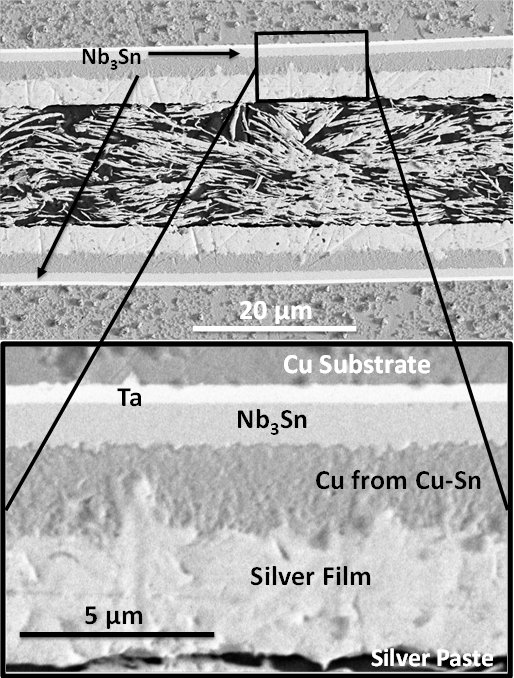
\includegraphics[width=.5\textwidth]{images/Cu/BronzeOnNb/BronzeOnNb.png}
        \caption[Recipe 3, Nb First: SEM Image of Nb$_3$Sn film made by depositing Nb onto a Cu substrate/Ta diffusion bilayer.]{Recipe 3, Nb First: SEM Image of Nb$_3$Sn film made by depositing Nb onto a Cu substrate/Ta diffusion bilayer. Then Cu-Sn was evaporated onto the Nb and post-reacted. This film had particularly uniform morphology due to the clean interface between Ta and Nb.}
        \label{fig:BronzeOnNb}
    \end{figure}

   % \begin{figure}
   %     \centering
   %    
\includegraphics[width=.7\textwidth]{images/Cu/ReactionComparisonwith.png}
   %     \caption[$T_c$ curves comparing post-reaction, hot-bronze, and hot-bronze + post-reaction]{Nb$_3$Sn transitions on Cu/Ta substrates comparing processing routes. Combined hot-bronze + post-reaction (blue, thin Cu-Sn first-recipe 1) achieves the sharpest transition ($\Delta T_c \sim 1$~K) versus hot bronze alone (black, $\Delta T_c \sim 1.5$~K) or post-reaction only (red, Nb first-recipe 3).}
   %     \label{fig:ReactionComparisonwith}
   % \end{figure}        
    

    
    